\documentclass{beamer}

\usepackage[utf8]{inputenc}
\usepackage{graphicx}
\usetheme{Berkeley} 
\usecolortheme{default}
\setbeamertemplate{footline}[frame number]

\title{Licence Pro ADSILLH}
 
\subtitle{GNOME-Games / GNOME-Music}
 
\author{Pierre-Antoine Rouby\\Gautier Delacour\\
  David Tabarie\\Kevin Carsoule\\Florian Darfeuille}

\date{Année 2017/2018}

\logo{
\includegraphics[width=1.5cm]{../images/logo_univ.jpg}}

% ce code permet d'afficher le sommaire à chaque section,
% en mettant en valeur la section courante (utile ?)
% \AtBeginSection[]
% {
%   \begin{frame}
%     \frametitle{Sommaire}
%     \tableofcontents[currentsection]
%   \end{frame}
% }

\begin{document}
\frame{\titlepage}

\begin{frame}
  \frametitle{Sommaire}
  \tableofcontents
\end{frame}

\section{Le projet GNOME}
\begin{frame}
  \frametitle{Le projet GNOME}
  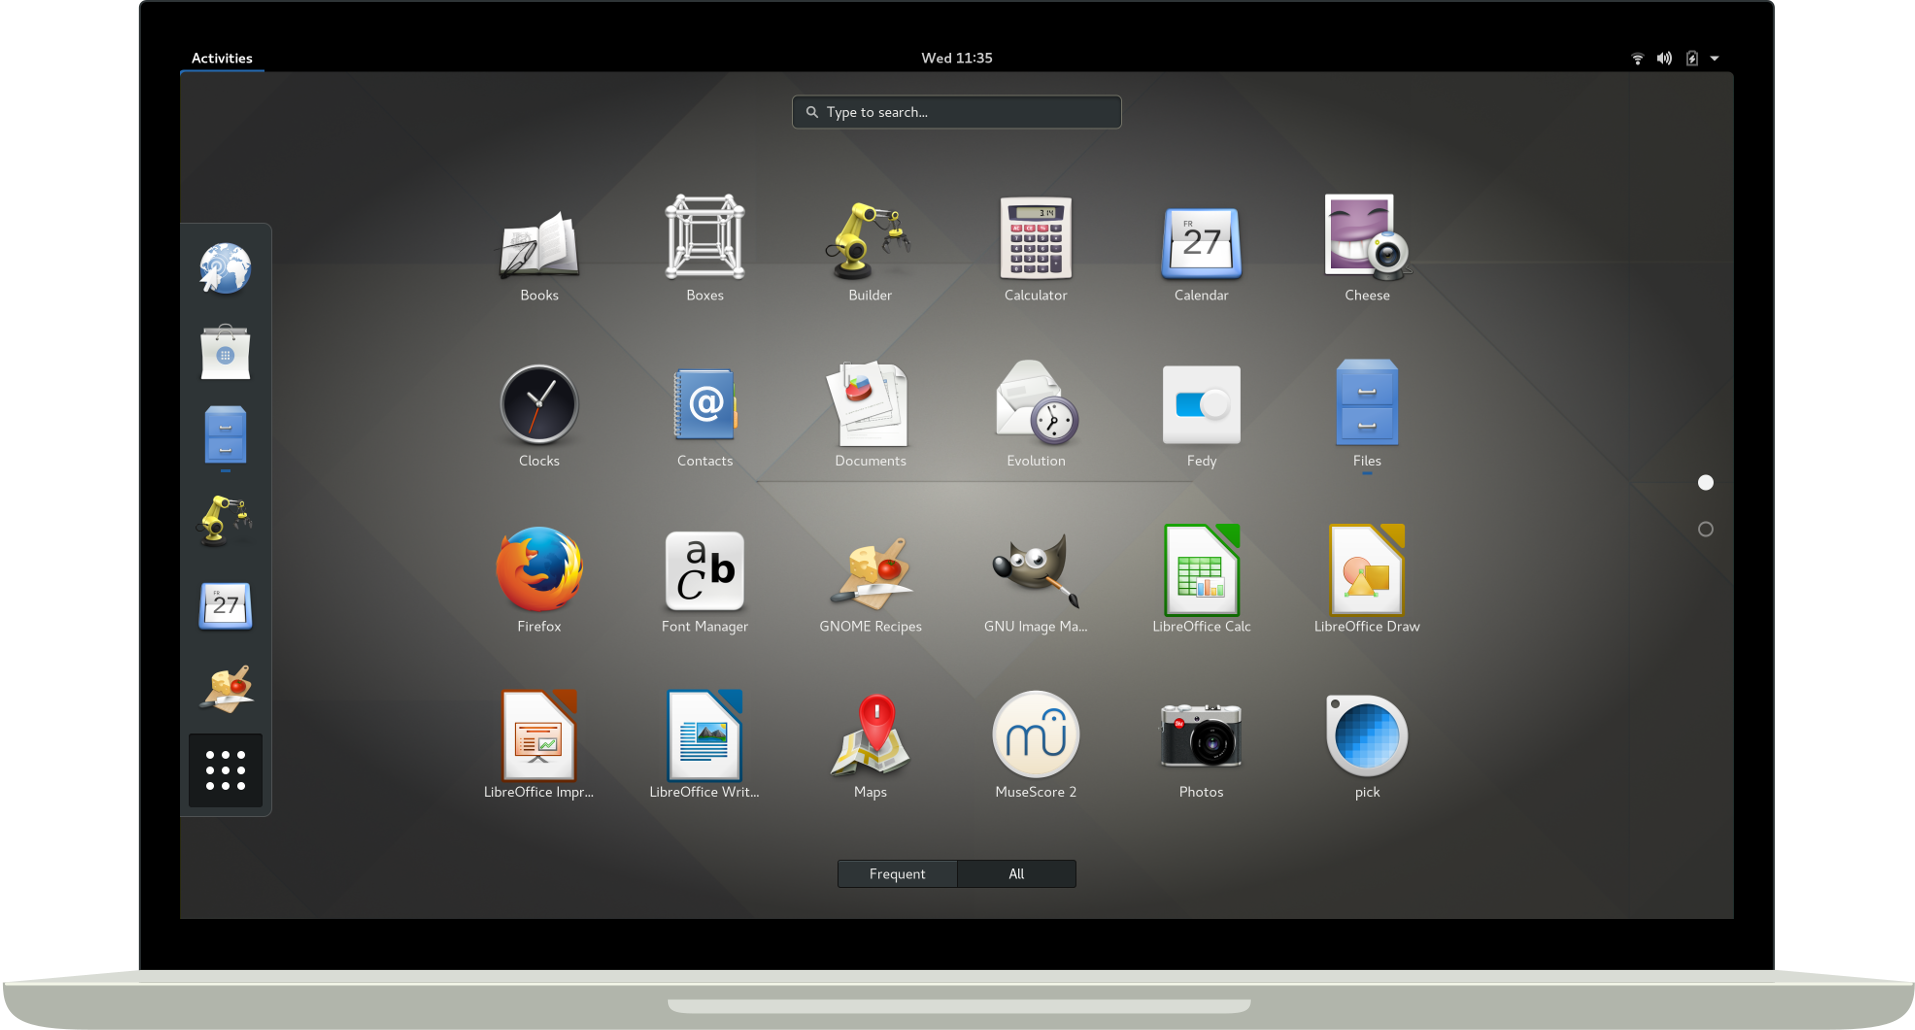
\includegraphics[scale=0.2]{images/GnomeScreen.png}
\end{frame}

\subsection{Les outils collaboratifs}
\begin{frame}
  \frametitle{Les outils collaboratifs}
  \begin{itemize}
  \item Bugzilla
  \item Wiki GNOME
  \item Git
  \item irc
  \end{itemize}
  \begin{figure}
    
\includegraphics[scale=0.1]{images/bugzilla-logo.png} \hspace{1cm}
    
\includegraphics[scale=0.04]{images/gnome-logo.png} \hspace{1cm}
    
\includegraphics[scale=0.03]{images/git-logo.png} \hspace{1cm}
    
\includegraphics[scale=0.07]{images/irc-logo.png}
  \end{figure}
  
  %% \begin{itemize}
  %% \item Bugzilla
  %%   
\includegraphics[scale=0.1]{images/bugzilla-logo.png}
  %% \item GnomeWiki
  %%   
\includegraphics[scale=0.04]{images/gnome-logo.png}
  %% \item Git
  %%   
\includegraphics[scale=0.03]{images/git-logo.png}
  %% \item IRC
  %%   
\includegraphics[scale=0.07]{images/irc-logo.png}
  %% \end{itemize}
\end{frame}

\subsection{Newcomers}
\begin{frame}
  \frametitle{Newcomers}
  \begin{itemize}
    \item Pour les nouveaux arrivant
    \item Channel irc dédié
  \end{itemize}
\end{frame}

\section{Le projet GNOME-Games}
\begin{frame}
  \frametitle{GNOME-Games}
  \includegraphics[scale=0.25]{images/screen-games.png}
\end{frame}

\subsection{Contributions effectués}
\begin{frame}
  \frametitle{Contributions effectués Games}
  \begin{itemize}
    \item Traçage d'un bug PulseAudio
    \item Patch : Modifications du fichier 'HACKING'
    \item Patch : Modifications du fichier 'README.md'
    \item Patch : Ajout d'un event 'retour au menu'
  \end{itemize}
\end{frame}

\subsection{Conclusion}
\begin{frame}
  \frametitle{Conclusion Games}
  \begin{itemize}
  \item Les outils collaboratifs
    \begin{itemize}
    \item Git
    \item irc
    \item Tracker de bug
    \end{itemize}
  \item Les prochaines contributions
  \end{itemize}
\end{frame}

\section{Le projet Gnome Music}
\begin{frame}
  \frametitle{Le projet Gnome Music}
\end{frame}

\subsection{Contributions effectués sur GNOME Music}
\begin{frame}
  \frametitle{Contributions effectuées}
  \begin{itemize}
  \item Rapport de bug sur le Builder
  \item Patch Pep8
  \item Patch Bouton retour arrière
  \end{itemize}
\end{frame}

\subsection{Conclusion Music}
\begin{frame}
  \frametitle{Conclusion Music}
\end{frame}

\section{Question}
\begin{frame}
  \frametitle{Question ?}
\end{frame}

\end{document}
